%-----------------------------------LICENSE------------------------------------%
%   This file is part of tikz_figures.                                         %
%                                                                              %
%   tikz_figures is free software: you can redistribute it and/or              %
%   modify it it under the terms of the GNU General Public License as          %
%   published by the Free Software Foundation, either version 3 of the         %
%   License, or (at your option) any later version.                            %
%                                                                              %
%   tikz_figures is distributed in the hope that it will be useful,            %
%   but WITHOUT ANY WARRANTY; without even the implied warranty of             %
%   MERCHANTABILITY or FITNESS FOR A PARTICULAR PURPOSE.  See the              %
%   GNU General Public License for more details.                               %
%                                                                              %
%   You should have received a copy of the GNU General Public License along    %
%   with tikz_figures.  If not, see <https://www.gnu.org/licenses/>.           %
%------------------------------------------------------------------------------%

% Use the standalone class for displaying the tikz image on a small PDF.
\documentclass[crop, tikz]{standalone}

% Import the tikz package to use for the drawing.
\usepackage{tikz}

% Needed for blackboard bold C.
\usepackage{amssymb}

% The arrow package is used for the LaTeX arrow.
\usetikzlibrary{arrows.meta}

% Begin the document.
\begin{document}

    % Draw the figure.
    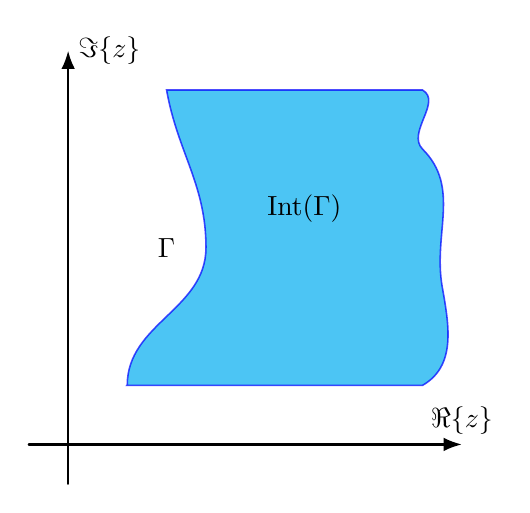
\begin{tikzpicture}[%
        > = Latex,
        line width = 0.2mm,
        line cap = round,
        scale = 2.5
    ]

        % Coordinates for the points that define the frame of the figure.
        \coordinate (P1) at (0.3, 0.3);
        \coordinate (P2) at (1.8, 0.3);
        \coordinate (P3) at (1.9, 0.8);
        \coordinate (P4) at (1.8, 1.5);
        \coordinate (P5) at (1.8, 1.8);
        \coordinate (P6) at (0.5, 1.8);
        \coordinate (P7) at (0.7, 1.0);

        % Axes:
        \begin{scope}[thick]
            \draw[->] (-0.2, 0) to (2, 0) node [above] {$\Re\{z\}$};
            \draw[->] (0, -0.2) to (0, 2) node [right] {$\Im\{z\}$};
        \end{scope}

        % Draw the simple region.
        \draw[blue,fill=cyan,opacity=0.7]
            (P1) to
            (P2) to [out = 30, in = -80]
            (P3) to [out = 100, in = -45]
            (P4) to [out = 135, in = -30]
            (P5) to
            (P6) to [out = -80, in = 90]
            (P7) to [out = -90, in = 90] cycle;

        % Nodes to label the Jordan curve and its interior.
        \node at (0.5,1)   {$\Gamma$};
        \node at (1.2,1.2) {$\textrm{Int}(\Gamma)$};
    \end{tikzpicture}
\end{document}
